\documentclass[11pt]{article}

    \usepackage[breakable]{tcolorbox}
    \usepackage{parskip} % Stop auto-indenting (to mimic markdown behaviour)
    

    % Basic figure setup, for now with no caption control since it's done
    % automatically by Pandoc (which extracts ![](path) syntax from Markdown).
    \usepackage{graphicx}
    % Maintain compatibility with old templates. Remove in nbconvert 6.0
    \let\Oldincludegraphics\includegraphics
    % Ensure that by default, figures have no caption (until we provide a
    % proper Figure object with a Caption API and a way to capture that
    % in the conversion process - todo).
    \usepackage{caption}
    \DeclareCaptionFormat{nocaption}{}
    \captionsetup{format=nocaption,aboveskip=0pt,belowskip=0pt}

    \usepackage{float}
    \floatplacement{figure}{H} % forces figures to be placed at the correct location
    \usepackage{xcolor} % Allow colors to be defined
    \usepackage{enumerate} % Needed for markdown enumerations to work
    \usepackage{geometry} % Used to adjust the document margins
    \usepackage{amsmath} % Equations
    \usepackage{amssymb} % Equations
    \usepackage{textcomp} % defines textquotesingle
    % Hack from http://tex.stackexchange.com/a/47451/13684:
    \AtBeginDocument{%
        \def\PYZsq{\textquotesingle}% Upright quotes in Pygmentized code
    }
    \usepackage{upquote} % Upright quotes for verbatim code
    \usepackage{eurosym} % defines \euro

    \usepackage{iftex}
    \ifPDFTeX
        \usepackage[T1]{fontenc}
        \IfFileExists{alphabeta.sty}{
              \usepackage{alphabeta}
          }{
              \usepackage[mathletters]{ucs}
              \usepackage[utf8x]{inputenc}
          }
    \else
        \usepackage{fontspec}
        \usepackage{unicode-math}
    \fi

    \usepackage{fancyvrb} % verbatim replacement that allows latex
    \usepackage{grffile} % extends the file name processing of package graphics
                         % to support a larger range
    \makeatletter % fix for old versions of grffile with XeLaTeX
    \@ifpackagelater{grffile}{2019/11/01}
    {
      % Do nothing on new versions
    }
    {
      \def\Gread@@xetex#1{%
        \IfFileExists{"\Gin@base".bb}%
        {\Gread@eps{\Gin@base.bb}}%
        {\Gread@@xetex@aux#1}%
      }
    }
    \makeatother
    \usepackage[Export]{adjustbox} % Used to constrain images to a maximum size
    \adjustboxset{max size={0.9\linewidth}{0.9\paperheight}}

    % The hyperref package gives us a pdf with properly built
    % internal navigation ('pdf bookmarks' for the table of contents,
    % internal cross-reference links, web links for URLs, etc.)
    \usepackage{hyperref}
    % The default LaTeX title has an obnoxious amount of whitespace. By default,
    % titling removes some of it. It also provides customization options.
    \usepackage{titling}
    \usepackage{longtable} % longtable support required by pandoc >1.10
    \usepackage{booktabs}  % table support for pandoc > 1.12.2
    \usepackage{array}     % table support for pandoc >= 2.11.3
    \usepackage{calc}      % table minipage width calculation for pandoc >= 2.11.1
    \usepackage[inline]{enumitem} % IRkernel/repr support (it uses the enumerate* environment)
    \usepackage[normalem]{ulem} % ulem is needed to support strikethroughs (\sout)
                                % normalem makes italics be italics, not underlines
    \usepackage{mathrsfs}
    

    
    % Colors for the hyperref package
    \definecolor{urlcolor}{rgb}{0,.145,.698}
    \definecolor{linkcolor}{rgb}{.71,0.21,0.01}
    \definecolor{citecolor}{rgb}{.12,.54,.11}

    % ANSI colors
    \definecolor{ansi-black}{HTML}{3E424D}
    \definecolor{ansi-black-intense}{HTML}{282C36}
    \definecolor{ansi-red}{HTML}{E75C58}
    \definecolor{ansi-red-intense}{HTML}{B22B31}
    \definecolor{ansi-green}{HTML}{00A250}
    \definecolor{ansi-green-intense}{HTML}{007427}
    \definecolor{ansi-yellow}{HTML}{DDB62B}
    \definecolor{ansi-yellow-intense}{HTML}{B27D12}
    \definecolor{ansi-blue}{HTML}{208FFB}
    \definecolor{ansi-blue-intense}{HTML}{0065CA}
    \definecolor{ansi-magenta}{HTML}{D160C4}
    \definecolor{ansi-magenta-intense}{HTML}{A03196}
    \definecolor{ansi-cyan}{HTML}{60C6C8}
    \definecolor{ansi-cyan-intense}{HTML}{258F8F}
    \definecolor{ansi-white}{HTML}{C5C1B4}
    \definecolor{ansi-white-intense}{HTML}{A1A6B2}
    \definecolor{ansi-default-inverse-fg}{HTML}{FFFFFF}
    \definecolor{ansi-default-inverse-bg}{HTML}{000000}

    % common color for the border for error outputs.
    \definecolor{outerrorbackground}{HTML}{FFDFDF}

    % commands and environments needed by pandoc snippets
    % extracted from the output of `pandoc -s`
    \providecommand{\tightlist}{%
      \setlength{\itemsep}{0pt}\setlength{\parskip}{0pt}}
    \DefineVerbatimEnvironment{Highlighting}{Verbatim}{commandchars=\\\{\}}
    % Add ',fontsize=\small' for more characters per line
    \newenvironment{Shaded}{}{}
    \newcommand{\KeywordTok}[1]{\textcolor[rgb]{0.00,0.44,0.13}{\textbf{{#1}}}}
    \newcommand{\DataTypeTok}[1]{\textcolor[rgb]{0.56,0.13,0.00}{{#1}}}
    \newcommand{\DecValTok}[1]{\textcolor[rgb]{0.25,0.63,0.44}{{#1}}}
    \newcommand{\BaseNTok}[1]{\textcolor[rgb]{0.25,0.63,0.44}{{#1}}}
    \newcommand{\FloatTok}[1]{\textcolor[rgb]{0.25,0.63,0.44}{{#1}}}
    \newcommand{\CharTok}[1]{\textcolor[rgb]{0.25,0.44,0.63}{{#1}}}
    \newcommand{\StringTok}[1]{\textcolor[rgb]{0.25,0.44,0.63}{{#1}}}
    \newcommand{\CommentTok}[1]{\textcolor[rgb]{0.38,0.63,0.69}{\textit{{#1}}}}
    \newcommand{\OtherTok}[1]{\textcolor[rgb]{0.00,0.44,0.13}{{#1}}}
    \newcommand{\AlertTok}[1]{\textcolor[rgb]{1.00,0.00,0.00}{\textbf{{#1}}}}
    \newcommand{\FunctionTok}[1]{\textcolor[rgb]{0.02,0.16,0.49}{{#1}}}
    \newcommand{\RegionMarkerTok}[1]{{#1}}
    \newcommand{\ErrorTok}[1]{\textcolor[rgb]{1.00,0.00,0.00}{\textbf{{#1}}}}
    \newcommand{\NormalTok}[1]{{#1}}

    % Additional commands for more recent versions of Pandoc
    \newcommand{\ConstantTok}[1]{\textcolor[rgb]{0.53,0.00,0.00}{{#1}}}
    \newcommand{\SpecialCharTok}[1]{\textcolor[rgb]{0.25,0.44,0.63}{{#1}}}
    \newcommand{\VerbatimStringTok}[1]{\textcolor[rgb]{0.25,0.44,0.63}{{#1}}}
    \newcommand{\SpecialStringTok}[1]{\textcolor[rgb]{0.73,0.40,0.53}{{#1}}}
    \newcommand{\ImportTok}[1]{{#1}}
    \newcommand{\DocumentationTok}[1]{\textcolor[rgb]{0.73,0.13,0.13}{\textit{{#1}}}}
    \newcommand{\AnnotationTok}[1]{\textcolor[rgb]{0.38,0.63,0.69}{\textbf{\textit{{#1}}}}}
    \newcommand{\CommentVarTok}[1]{\textcolor[rgb]{0.38,0.63,0.69}{\textbf{\textit{{#1}}}}}
    \newcommand{\VariableTok}[1]{\textcolor[rgb]{0.10,0.09,0.49}{{#1}}}
    \newcommand{\ControlFlowTok}[1]{\textcolor[rgb]{0.00,0.44,0.13}{\textbf{{#1}}}}
    \newcommand{\OperatorTok}[1]{\textcolor[rgb]{0.40,0.40,0.40}{{#1}}}
    \newcommand{\BuiltInTok}[1]{{#1}}
    \newcommand{\ExtensionTok}[1]{{#1}}
    \newcommand{\PreprocessorTok}[1]{\textcolor[rgb]{0.74,0.48,0.00}{{#1}}}
    \newcommand{\AttributeTok}[1]{\textcolor[rgb]{0.49,0.56,0.16}{{#1}}}
    \newcommand{\InformationTok}[1]{\textcolor[rgb]{0.38,0.63,0.69}{\textbf{\textit{{#1}}}}}
    \newcommand{\WarningTok}[1]{\textcolor[rgb]{0.38,0.63,0.69}{\textbf{\textit{{#1}}}}}


    % Define a nice break command that doesn't care if a line doesn't already
    % exist.
    \def\br{\hspace*{\fill} \\* }
    % Math Jax compatibility definitions
    \def\gt{>}
    \def\lt{<}
    \let\Oldtex\TeX
    \let\Oldlatex\LaTeX
    \renewcommand{\TeX}{\textrm{\Oldtex}}
    \renewcommand{\LaTeX}{\textrm{\Oldlatex}}
    % Document parameters
    % Document title
    \title{Analisi Esperimenti Ca214}
    
    
    
    
    
% Pygments definitions
\makeatletter
\def\PY@reset{\let\PY@it=\relax \let\PY@bf=\relax%
    \let\PY@ul=\relax \let\PY@tc=\relax%
    \let\PY@bc=\relax \let\PY@ff=\relax}
\def\PY@tok#1{\csname PY@tok@#1\endcsname}
\def\PY@toks#1+{\ifx\relax#1\empty\else%
    \PY@tok{#1}\expandafter\PY@toks\fi}
\def\PY@do#1{\PY@bc{\PY@tc{\PY@ul{%
    \PY@it{\PY@bf{\PY@ff{#1}}}}}}}
\def\PY#1#2{\PY@reset\PY@toks#1+\relax+\PY@do{#2}}

\expandafter\def\csname PY@tok@w\endcsname{\def\PY@tc##1{\textcolor[rgb]{0.73,0.73,0.73}{##1}}}
\expandafter\def\csname PY@tok@c\endcsname{\let\PY@it=\textit\def\PY@tc##1{\textcolor[rgb]{0.25,0.50,0.50}{##1}}}
\expandafter\def\csname PY@tok@cp\endcsname{\def\PY@tc##1{\textcolor[rgb]{0.74,0.48,0.00}{##1}}}
\expandafter\def\csname PY@tok@k\endcsname{\let\PY@bf=\textbf\def\PY@tc##1{\textcolor[rgb]{0.00,0.50,0.00}{##1}}}
\expandafter\def\csname PY@tok@kp\endcsname{\def\PY@tc##1{\textcolor[rgb]{0.00,0.50,0.00}{##1}}}
\expandafter\def\csname PY@tok@kt\endcsname{\def\PY@tc##1{\textcolor[rgb]{0.69,0.00,0.25}{##1}}}
\expandafter\def\csname PY@tok@o\endcsname{\def\PY@tc##1{\textcolor[rgb]{0.40,0.40,0.40}{##1}}}
\expandafter\def\csname PY@tok@ow\endcsname{\let\PY@bf=\textbf\def\PY@tc##1{\textcolor[rgb]{0.67,0.13,1.00}{##1}}}
\expandafter\def\csname PY@tok@nb\endcsname{\def\PY@tc##1{\textcolor[rgb]{0.00,0.50,0.00}{##1}}}
\expandafter\def\csname PY@tok@nf\endcsname{\def\PY@tc##1{\textcolor[rgb]{0.00,0.00,1.00}{##1}}}
\expandafter\def\csname PY@tok@nc\endcsname{\let\PY@bf=\textbf\def\PY@tc##1{\textcolor[rgb]{0.00,0.00,1.00}{##1}}}
\expandafter\def\csname PY@tok@nn\endcsname{\let\PY@bf=\textbf\def\PY@tc##1{\textcolor[rgb]{0.00,0.00,1.00}{##1}}}
\expandafter\def\csname PY@tok@ne\endcsname{\let\PY@bf=\textbf\def\PY@tc##1{\textcolor[rgb]{0.82,0.25,0.23}{##1}}}
\expandafter\def\csname PY@tok@nv\endcsname{\def\PY@tc##1{\textcolor[rgb]{0.10,0.09,0.49}{##1}}}
\expandafter\def\csname PY@tok@no\endcsname{\def\PY@tc##1{\textcolor[rgb]{0.53,0.00,0.00}{##1}}}
\expandafter\def\csname PY@tok@nl\endcsname{\def\PY@tc##1{\textcolor[rgb]{0.63,0.63,0.00}{##1}}}
\expandafter\def\csname PY@tok@ni\endcsname{\let\PY@bf=\textbf\def\PY@tc##1{\textcolor[rgb]{0.60,0.60,0.60}{##1}}}
\expandafter\def\csname PY@tok@na\endcsname{\def\PY@tc##1{\textcolor[rgb]{0.49,0.56,0.16}{##1}}}
\expandafter\def\csname PY@tok@nt\endcsname{\let\PY@bf=\textbf\def\PY@tc##1{\textcolor[rgb]{0.00,0.50,0.00}{##1}}}
\expandafter\def\csname PY@tok@nd\endcsname{\def\PY@tc##1{\textcolor[rgb]{0.67,0.13,1.00}{##1}}}
\expandafter\def\csname PY@tok@s\endcsname{\def\PY@tc##1{\textcolor[rgb]{0.73,0.13,0.13}{##1}}}
\expandafter\def\csname PY@tok@sd\endcsname{\let\PY@it=\textit\def\PY@tc##1{\textcolor[rgb]{0.73,0.13,0.13}{##1}}}
\expandafter\def\csname PY@tok@si\endcsname{\let\PY@bf=\textbf\def\PY@tc##1{\textcolor[rgb]{0.73,0.40,0.53}{##1}}}
\expandafter\def\csname PY@tok@se\endcsname{\let\PY@bf=\textbf\def\PY@tc##1{\textcolor[rgb]{0.73,0.40,0.13}{##1}}}
\expandafter\def\csname PY@tok@sr\endcsname{\def\PY@tc##1{\textcolor[rgb]{0.73,0.40,0.53}{##1}}}
\expandafter\def\csname PY@tok@ss\endcsname{\def\PY@tc##1{\textcolor[rgb]{0.10,0.09,0.49}{##1}}}
\expandafter\def\csname PY@tok@sx\endcsname{\def\PY@tc##1{\textcolor[rgb]{0.00,0.50,0.00}{##1}}}
\expandafter\def\csname PY@tok@m\endcsname{\def\PY@tc##1{\textcolor[rgb]{0.40,0.40,0.40}{##1}}}
\expandafter\def\csname PY@tok@gh\endcsname{\let\PY@bf=\textbf\def\PY@tc##1{\textcolor[rgb]{0.00,0.00,0.50}{##1}}}
\expandafter\def\csname PY@tok@gu\endcsname{\let\PY@bf=\textbf\def\PY@tc##1{\textcolor[rgb]{0.50,0.00,0.50}{##1}}}
\expandafter\def\csname PY@tok@gd\endcsname{\def\PY@tc##1{\textcolor[rgb]{0.63,0.00,0.00}{##1}}}
\expandafter\def\csname PY@tok@gi\endcsname{\def\PY@tc##1{\textcolor[rgb]{0.00,0.63,0.00}{##1}}}
\expandafter\def\csname PY@tok@gr\endcsname{\def\PY@tc##1{\textcolor[rgb]{1.00,0.00,0.00}{##1}}}
\expandafter\def\csname PY@tok@ge\endcsname{\let\PY@it=\textit}
\expandafter\def\csname PY@tok@gs\endcsname{\let\PY@bf=\textbf}
\expandafter\def\csname PY@tok@gp\endcsname{\let\PY@bf=\textbf\def\PY@tc##1{\textcolor[rgb]{0.00,0.00,0.50}{##1}}}
\expandafter\def\csname PY@tok@go\endcsname{\def\PY@tc##1{\textcolor[rgb]{0.53,0.53,0.53}{##1}}}
\expandafter\def\csname PY@tok@gt\endcsname{\def\PY@tc##1{\textcolor[rgb]{0.00,0.27,0.87}{##1}}}
\expandafter\def\csname PY@tok@err\endcsname{\def\PY@bc##1{\setlength{\fboxsep}{0pt}\fcolorbox[rgb]{1.00,0.00,0.00}{1,1,1}{\strut ##1}}}
\expandafter\def\csname PY@tok@kc\endcsname{\let\PY@bf=\textbf\def\PY@tc##1{\textcolor[rgb]{0.00,0.50,0.00}{##1}}}
\expandafter\def\csname PY@tok@kd\endcsname{\let\PY@bf=\textbf\def\PY@tc##1{\textcolor[rgb]{0.00,0.50,0.00}{##1}}}
\expandafter\def\csname PY@tok@kn\endcsname{\let\PY@bf=\textbf\def\PY@tc##1{\textcolor[rgb]{0.00,0.50,0.00}{##1}}}
\expandafter\def\csname PY@tok@kr\endcsname{\let\PY@bf=\textbf\def\PY@tc##1{\textcolor[rgb]{0.00,0.50,0.00}{##1}}}
\expandafter\def\csname PY@tok@bp\endcsname{\def\PY@tc##1{\textcolor[rgb]{0.00,0.50,0.00}{##1}}}
\expandafter\def\csname PY@tok@fm\endcsname{\def\PY@tc##1{\textcolor[rgb]{0.00,0.00,1.00}{##1}}}
\expandafter\def\csname PY@tok@vc\endcsname{\def\PY@tc##1{\textcolor[rgb]{0.10,0.09,0.49}{##1}}}
\expandafter\def\csname PY@tok@vg\endcsname{\def\PY@tc##1{\textcolor[rgb]{0.10,0.09,0.49}{##1}}}
\expandafter\def\csname PY@tok@vi\endcsname{\def\PY@tc##1{\textcolor[rgb]{0.10,0.09,0.49}{##1}}}
\expandafter\def\csname PY@tok@vm\endcsname{\def\PY@tc##1{\textcolor[rgb]{0.10,0.09,0.49}{##1}}}
\expandafter\def\csname PY@tok@sa\endcsname{\def\PY@tc##1{\textcolor[rgb]{0.73,0.13,0.13}{##1}}}
\expandafter\def\csname PY@tok@sb\endcsname{\def\PY@tc##1{\textcolor[rgb]{0.73,0.13,0.13}{##1}}}
\expandafter\def\csname PY@tok@sc\endcsname{\def\PY@tc##1{\textcolor[rgb]{0.73,0.13,0.13}{##1}}}
\expandafter\def\csname PY@tok@dl\endcsname{\def\PY@tc##1{\textcolor[rgb]{0.73,0.13,0.13}{##1}}}
\expandafter\def\csname PY@tok@s2\endcsname{\def\PY@tc##1{\textcolor[rgb]{0.73,0.13,0.13}{##1}}}
\expandafter\def\csname PY@tok@sh\endcsname{\def\PY@tc##1{\textcolor[rgb]{0.73,0.13,0.13}{##1}}}
\expandafter\def\csname PY@tok@s1\endcsname{\def\PY@tc##1{\textcolor[rgb]{0.73,0.13,0.13}{##1}}}
\expandafter\def\csname PY@tok@mb\endcsname{\def\PY@tc##1{\textcolor[rgb]{0.40,0.40,0.40}{##1}}}
\expandafter\def\csname PY@tok@mf\endcsname{\def\PY@tc##1{\textcolor[rgb]{0.40,0.40,0.40}{##1}}}
\expandafter\def\csname PY@tok@mh\endcsname{\def\PY@tc##1{\textcolor[rgb]{0.40,0.40,0.40}{##1}}}
\expandafter\def\csname PY@tok@mi\endcsname{\def\PY@tc##1{\textcolor[rgb]{0.40,0.40,0.40}{##1}}}
\expandafter\def\csname PY@tok@il\endcsname{\def\PY@tc##1{\textcolor[rgb]{0.40,0.40,0.40}{##1}}}
\expandafter\def\csname PY@tok@mo\endcsname{\def\PY@tc##1{\textcolor[rgb]{0.40,0.40,0.40}{##1}}}
\expandafter\def\csname PY@tok@ch\endcsname{\let\PY@it=\textit\def\PY@tc##1{\textcolor[rgb]{0.25,0.50,0.50}{##1}}}
\expandafter\def\csname PY@tok@cm\endcsname{\let\PY@it=\textit\def\PY@tc##1{\textcolor[rgb]{0.25,0.50,0.50}{##1}}}
\expandafter\def\csname PY@tok@cpf\endcsname{\let\PY@it=\textit\def\PY@tc##1{\textcolor[rgb]{0.25,0.50,0.50}{##1}}}
\expandafter\def\csname PY@tok@c1\endcsname{\let\PY@it=\textit\def\PY@tc##1{\textcolor[rgb]{0.25,0.50,0.50}{##1}}}
\expandafter\def\csname PY@tok@cs\endcsname{\let\PY@it=\textit\def\PY@tc##1{\textcolor[rgb]{0.25,0.50,0.50}{##1}}}

\def\PYZbs{\char`\\}
\def\PYZus{\char`\_}
\def\PYZob{\char`\{}
\def\PYZcb{\char`\}}
\def\PYZca{\char`\^}
\def\PYZam{\char`\&}
\def\PYZlt{\char`\<}
\def\PYZgt{\char`\>}
\def\PYZsh{\char`\#}
\def\PYZpc{\char`\%}
\def\PYZdl{\char`\$}
\def\PYZhy{\char`\-}
\def\PYZsq{\char`\'}
\def\PYZdq{\char`\"}
\def\PYZti{\char`\~}
% for compatibility with earlier versions
\def\PYZat{@}
\def\PYZlb{[}
\def\PYZrb{]}
\makeatother


    % For linebreaks inside Verbatim environment from package fancyvrb.
    \makeatletter
        \newbox\Wrappedcontinuationbox
        \newbox\Wrappedvisiblespacebox
        \newcommand*\Wrappedvisiblespace {\textcolor{red}{\textvisiblespace}}
        \newcommand*\Wrappedcontinuationsymbol {\textcolor{red}{\llap{\tiny$\m@th\hookrightarrow$}}}
        \newcommand*\Wrappedcontinuationindent {3ex }
        \newcommand*\Wrappedafterbreak {\kern\Wrappedcontinuationindent\copy\Wrappedcontinuationbox}
        % Take advantage of the already applied Pygments mark-up to insert
        % potential linebreaks for TeX processing.
        %        {, <, #, %, $, ' and ": go to next line.
        %        _, }, ^, &, >, - and ~: stay at end of broken line.
        % Use of \textquotesingle for straight quote.
        \newcommand*\Wrappedbreaksatspecials {%
            \def\PYGZus{\discretionary{\char`\_}{\Wrappedafterbreak}{\char`\_}}%
            \def\PYGZob{\discretionary{}{\Wrappedafterbreak\char`\{}{\char`\{}}%
            \def\PYGZcb{\discretionary{\char`\}}{\Wrappedafterbreak}{\char`\}}}%
            \def\PYGZca{\discretionary{\char`\^}{\Wrappedafterbreak}{\char`\^}}%
            \def\PYGZam{\discretionary{\char`\&}{\Wrappedafterbreak}{\char`\&}}%
            \def\PYGZlt{\discretionary{}{\Wrappedafterbreak\char`\<}{\char`\<}}%
            \def\PYGZgt{\discretionary{\char`\>}{\Wrappedafterbreak}{\char`\>}}%
            \def\PYGZsh{\discretionary{}{\Wrappedafterbreak\char`\#}{\char`\#}}%
            \def\PYGZpc{\discretionary{}{\Wrappedafterbreak\char`\%}{\char`\%}}%
            \def\PYGZdl{\discretionary{}{\Wrappedafterbreak\char`\$}{\char`\$}}%
            \def\PYGZhy{\discretionary{\char`\-}{\Wrappedafterbreak}{\char`\-}}%
            \def\PYGZsq{\discretionary{}{\Wrappedafterbreak\textquotesingle}{\textquotesingle}}%
            \def\PYGZdq{\discretionary{}{\Wrappedafterbreak\char`\"}{\char`\"}}%
            \def\PYGZti{\discretionary{\char`\~}{\Wrappedafterbreak}{\char`\~}}%
        }
        % Some characters . , ; ? ! / are not pygmentized.
        % This macro makes them "active" and they will insert potential linebreaks
        \newcommand*\Wrappedbreaksatpunct {%
            \lccode`\~`\.\lowercase{\def~}{\discretionary{\hbox{\char`\.}}{\Wrappedafterbreak}{\hbox{\char`\.}}}%
            \lccode`\~`\,\lowercase{\def~}{\discretionary{\hbox{\char`\,}}{\Wrappedafterbreak}{\hbox{\char`\,}}}%
            \lccode`\~`\;\lowercase{\def~}{\discretionary{\hbox{\char`\;}}{\Wrappedafterbreak}{\hbox{\char`\;}}}%
            \lccode`\~`\:\lowercase{\def~}{\discretionary{\hbox{\char`\:}}{\Wrappedafterbreak}{\hbox{\char`\:}}}%
            \lccode`\~`\?\lowercase{\def~}{\discretionary{\hbox{\char`\?}}{\Wrappedafterbreak}{\hbox{\char`\?}}}%
            \lccode`\~`\!\lowercase{\def~}{\discretionary{\hbox{\char`\!}}{\Wrappedafterbreak}{\hbox{\char`\!}}}%
            \lccode`\~`\/\lowercase{\def~}{\discretionary{\hbox{\char`\/}}{\Wrappedafterbreak}{\hbox{\char`\/}}}%
            \catcode`\.\active
            \catcode`\,\active
            \catcode`\;\active
            \catcode`\:\active
            \catcode`\?\active
            \catcode`\!\active
            \catcode`\/\active
            \lccode`\~`\~
        }
    \makeatother

    \let\OriginalVerbatim=\Verbatim
    \makeatletter
    \renewcommand{\Verbatim}[1][1]{%
        %\parskip\z@skip
        \sbox\Wrappedcontinuationbox {\Wrappedcontinuationsymbol}%
        \sbox\Wrappedvisiblespacebox {\FV@SetupFont\Wrappedvisiblespace}%
        \def\FancyVerbFormatLine ##1{\hsize\linewidth
            \vtop{\raggedright\hyphenpenalty\z@\exhyphenpenalty\z@
                \doublehyphendemerits\z@\finalhyphendemerits\z@
                \strut ##1\strut}%
        }%
        % If the linebreak is at a space, the latter will be displayed as visible
        % space at end of first line, and a continuation symbol starts next line.
        % Stretch/shrink are however usually zero for typewriter font.
        \def\FV@Space {%
            \nobreak\hskip\z@ plus\fontdimen3\font minus\fontdimen4\font
            \discretionary{\copy\Wrappedvisiblespacebox}{\Wrappedafterbreak}
            {\kern\fontdimen2\font}%
        }%

        % Allow breaks at special characters using \PYG... macros.
        \Wrappedbreaksatspecials
        % Breaks at punctuation characters . , ; ? ! and / need catcode=\active
        \OriginalVerbatim[#1,codes*=\Wrappedbreaksatpunct]%
    }
    \makeatother

    % Exact colors from NB
    \definecolor{incolor}{HTML}{303F9F}
    \definecolor{outcolor}{HTML}{D84315}
    \definecolor{cellborder}{HTML}{CFCFCF}
    \definecolor{cellbackground}{HTML}{F7F7F7}

    % prompt
    \makeatletter
    \newcommand{\boxspacing}{\kern\kvtcb@left@rule\kern\kvtcb@boxsep}
    \makeatother
    \newcommand{\prompt}[4]{
        {\ttfamily\llap{{\color{#2}[#3]:\hspace{3pt}#4}}\vspace{-\baselineskip}}
    }
    

    
    % Prevent overflowing lines due to hard-to-break entities
    \sloppy
    % Setup hyperref package
    \hypersetup{
      breaklinks=true,  % so long urls are correctly broken across lines
      colorlinks=true,
      urlcolor=urlcolor,
      linkcolor=linkcolor,
      citecolor=citecolor,
      }
    % Slightly bigger margins than the latex defaults
    
    \geometry{verbose,tmargin=1in,bmargin=1in,lmargin=1in,rmargin=1in}
    
    

\begin{document}
    
    \maketitle
    
    

    
    \hypertarget{esperimenti}{%
\section{Esperimenti}\label{esperimenti}}

    Foglio di sintesi degli esperimenti effettuati su campioni di Ca214 per
la caratterizzazione elettrica. La caratterizzazione è realizzata con
connessione a 2-fili iniettando corrente lungo l'asse C e misurando la
tensione risultante in funzione della temperatura. Gli esperimenti sono
effettuati sia con corrente costante che variabile nella forma di una
rampa lineare o di onda quadra.

    \hypertarget{strumentazione}{%
\subsection{Strumentazione}\label{strumentazione}}

Negli esperimenti sono stati utilizzati due diversi generatori di
corrente i modelli 2400 e 6221 della Keithley Inc.~e come voltmetro il
modello 2182A sempre della Keithley Inc., montati secondo lo schema
seguente:

\begin{figure}
\centering
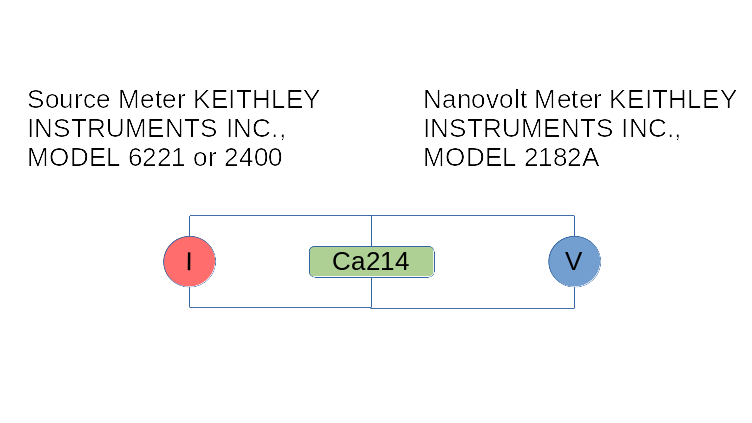
\includegraphics{schema_collegamenti.png}
\caption{schema collegamenti}
\end{figure}

La temperatura è stata misurata con un sensore al Si modello DT-400
della LakeShore collegato al multimetro della Keithley modello 2700.

    \hypertarget{realizzazione-dei-contatti}{%
\subsection{Realizzazione dei
Contatti}\label{realizzazione-dei-contatti}}

I contatti sul cristallo sono stati realizzati a freddo usando una pasta
saldante a base di Ag, sono state sperimentate due diverse paste
saldanti.

Esempio di contatto su CA12X\_C5:

\begin{figure}
\centering
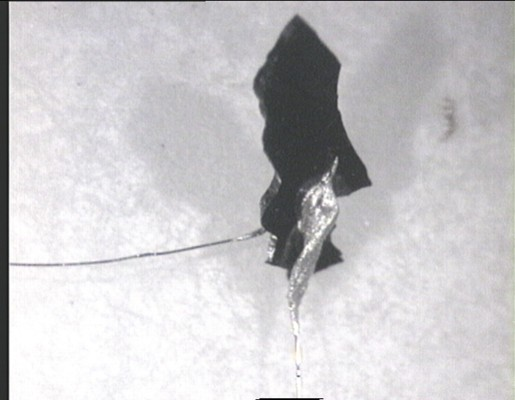
\includegraphics[width=50mm,scale=0.5]{ca12x_c5_saldatura_lato_b.jpg}
\caption{Esempio saldatura}
\end{figure}

Per alcuni cristalli è stata creata una piazzola depositando Ag su
entrambe le facce con il metodo della polverizzazione catodica per
migliorare la qualità del contatto.

Esempio di deposizione su CA12X2\_C1:

\begin{figure}
\centering
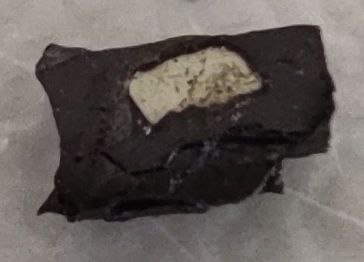
\includegraphics[width=50mm,scale=0.5]{ca12x2_c1_deposizione_argento.jpeg}
\caption{Esempio deposizione Ag}
\end{figure}

    \hypertarget{esempi-di-caratteristica}{%
\subsection{Esempi di caratteristica}\label{esempi-di-caratteristica}}

Esperimento su campione di \textbf{CA15A} a corrente variabile a
temperatura di \textbf{295°K}:

\begin{figure}
\centering
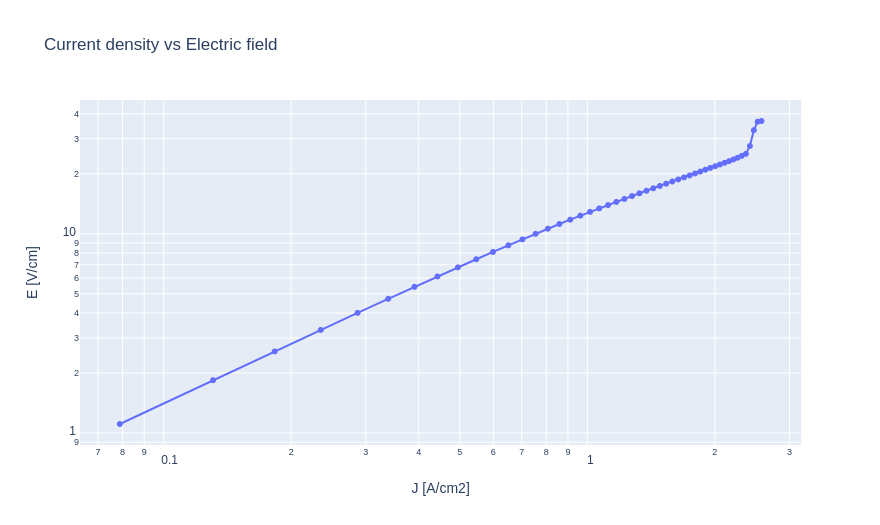
\includegraphics{CA15A_current_from_12e-3_to_400e-3A-20220321120002.png}
\caption{Esperimento
CA15A\_current\_from\_12e-3\_to\_400e-3A-20220321120002}
\end{figure}

Esperimento su campione di \textbf{CPRO\_03\_CE2\_A1} a temperatura
variabile e corrente di \textbf{30uA}:

\begin{figure}
\centering
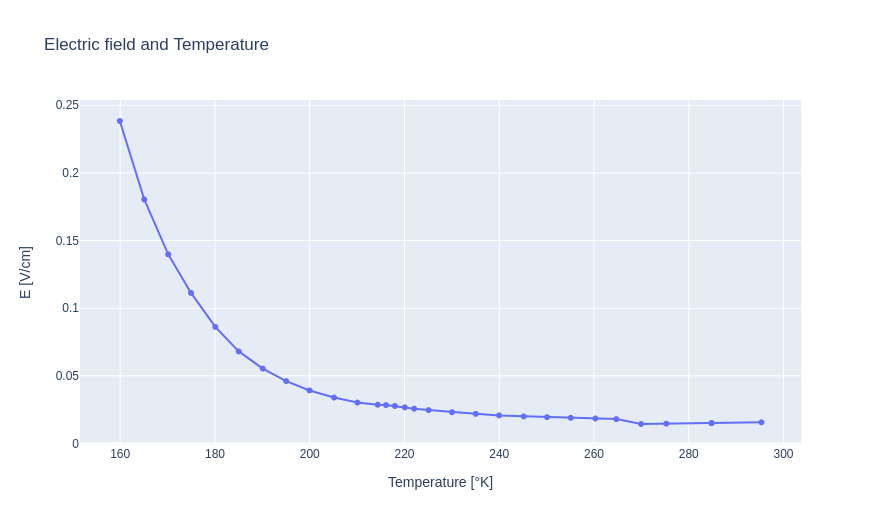
\includegraphics{CPRO_03_CE2_A1_at_fixed_current_30e-6A-20220414154149.png}
\caption{Esperimento
CPRO\_03\_CE2\_A1\_at\_fixed\_current\_30e-6A-20220414154149}
\end{figure}

    \hypertarget{oscillazioni-del-campo-elettrico}{%
\subsection{Oscillazioni del campo
elettrico}\label{oscillazioni-del-campo-elettrico}}

Durante le sperimentazioni, per alcuni cristalli (si vedano i paragrafi
1.4 e 1.5), si è misurata un'oscillazione del campo elettrico in certe
condizioni di temperatura e corrente. Il fenomeno è stato registrato con
diverse strumentazioni e modalità di contatti e si è evidenziato a
\textbf{temperature inferiori di 130°K} e per \textbf{densità di
corrente inferiori a 100 uA/cm2}.

Di queste oscillazioni sono state misurate l'ampiezza e il periodo
riscontrando per queste grandezze un intervallo di \textbf{{[}˜100,
˜450{]}V/cm} per la prima e \textbf{{[}˜2000, ˜2800{]}ms} per la
seconda, si veda il paragrafo 3.1.4. Il valore inferiore di ˜2s del
periodo potrebbe dipendere dai limiti del sistema di misurazione.

Dalla valutazione complessiva dei dati non si evidenzia alcuna
correlazione diretta del periodo e dell'ampiezza delle oscillazioni con
la temperatura e la densità di corrente, si consultino le matrici di
correlazione della sezione 4.

    \hypertarget{innesco-dovuto-alla-temperatura}{%
\subsubsection{Innesco dovuto alla
temperatura}\label{innesco-dovuto-alla-temperatura}}

Esempio dell'innesco delle oscillazioni per effetto della temperatura
sul campione di cristallo \textbf{CA12\_01\_A}. L'esperimento
CA12\_01\_A\_current\_from\_1e-7\_to\_10e-7A-2022042914575 consiste
nella polarizzazione del campione con una rampa di corrente da
\textbf{0.1uA a 1uA} ripetuta per quattro volte con la temperatura che
parte da \textbf{137.67°K} e scende fino a \textbf{126.56°K}. Le prime
due rampe di corrente non presentano oscillazioni, la terza presenta
oscillazioni appena la temperatura scende sotto 130°K, oscillazioni che
si ripresentano nella quarta e ultima rampa. In quest'ultima la
temperatura è più bassa e l'innesco avviene a una corrente più bassa
rispetto alla rampa precedente.

\begin{figure}
\centering
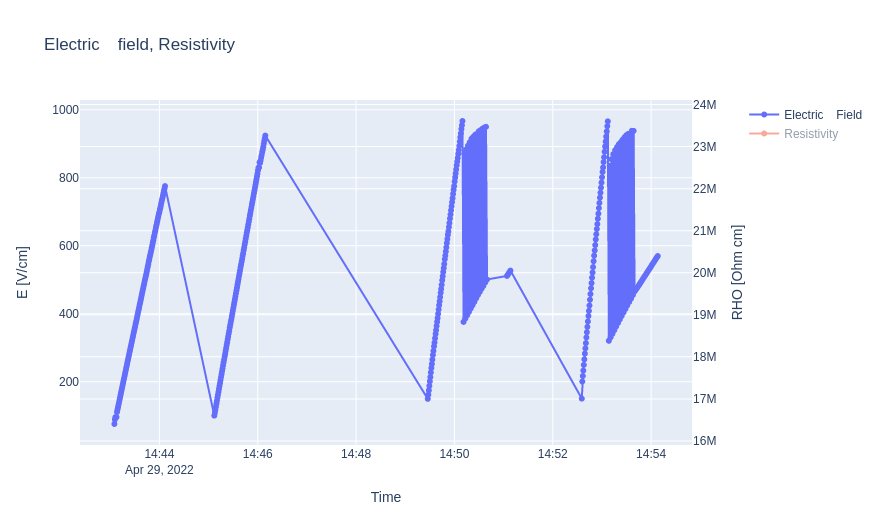
\includegraphics{ca12_01_a-e.png}
\caption{Ca12\_01\_A}
\end{figure}

\begin{figure}
\centering
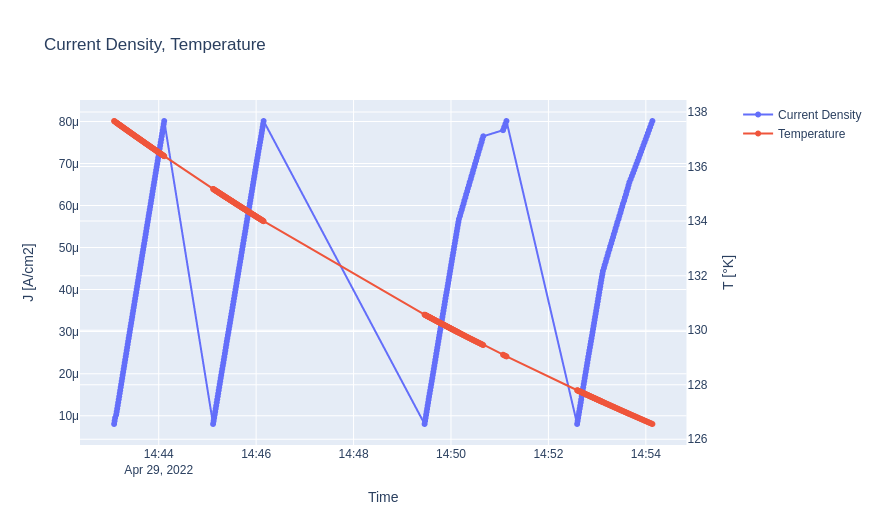
\includegraphics{ca12_01_a-j_t.png}
\caption{Ca12\_01\_A}
\end{figure}

È da notare che la pendenza della densità di corrente si riduce
all'innesco delle oscillazioni, questo aspetto è comune a tutti gli
esperimenti con rampa.

    \hypertarget{innesco-dovuto-alla-corrente}{%
\subsubsection{Innesco dovuto alla
corrente}\label{innesco-dovuto-alla-corrente}}

In questo caso è preso in esame il campione \textbf{CA12X\_C5}
polarizzato con corrente costante con una sequenza di esperimenti alla
temperatura di \textbf{113°K}

Esperimento CA12X\_C5\_at\_fixed\_current\_1e-7A-20220413144028 con
corrente costante di \textbf{0.1uA}, non presenta oscillazioni del campo
elettrico

\begin{figure}
\centering
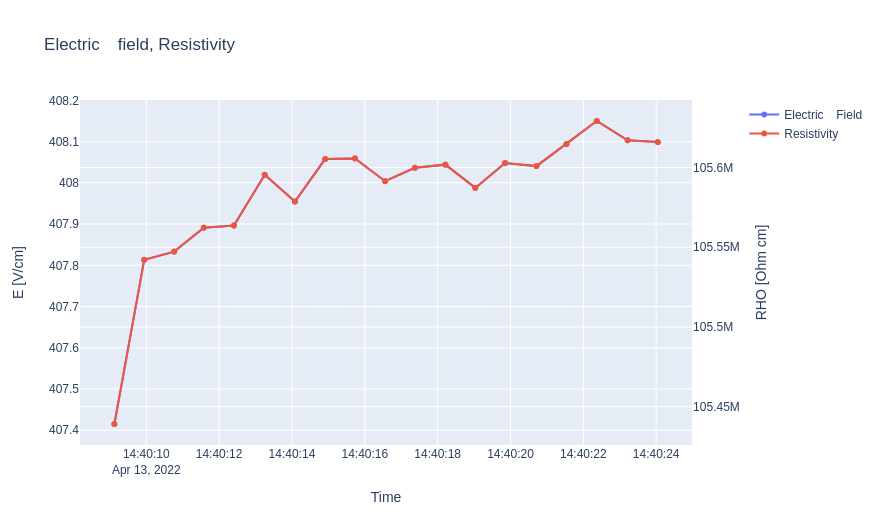
\includegraphics{CA12X_C5-1.png}
\caption{CA12X\_C5}
\end{figure}

Esperimento CA12X\_C5\_at\_fixed\_current\_2e-7A-20220413144122 con
corrente costante di \textbf{0.2uA}, non presenta oscillazioni del campo
elettrico

\begin{figure}
\centering
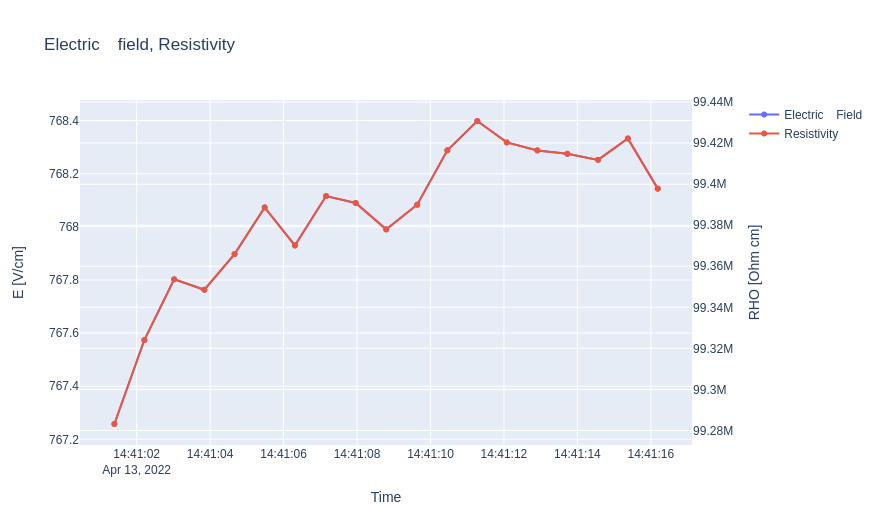
\includegraphics{CA12X_C5-2.png}
\caption{CA12X\_C5}
\end{figure}

Presenza delle oscillazioni nell'esperimento
CA12X\_C5\_at\_fixed\_current\_3e-7A-20220413144233 con corrente
costante di \textbf{0.3uA}

\begin{figure}
\centering
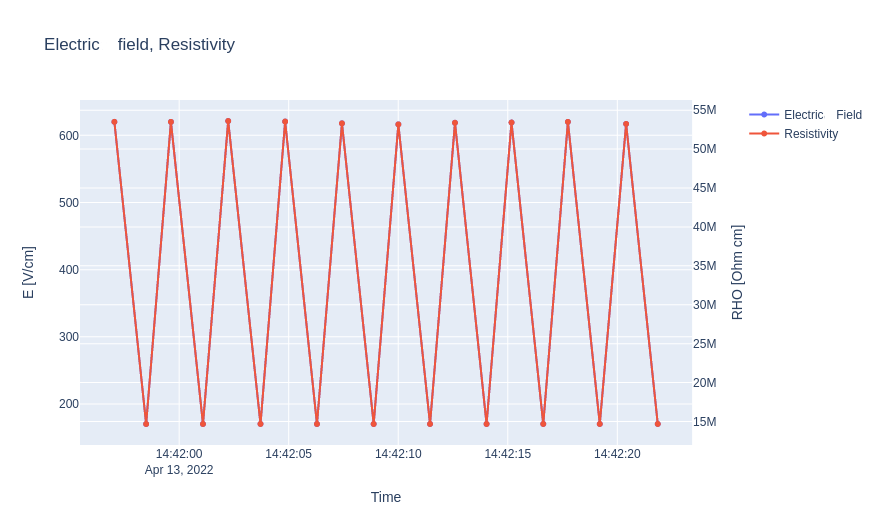
\includegraphics{CA12X_C5-3.png}
\caption{CA12X\_C5}
\end{figure}

Presenza ancora delle oscillazioni nell'esperimento
CA12X\_C5\_at\_fixed\_current\_3.5e-7A-20220413144545 con corrente
costante di \textbf{0.35uA}

\begin{figure}
\centering
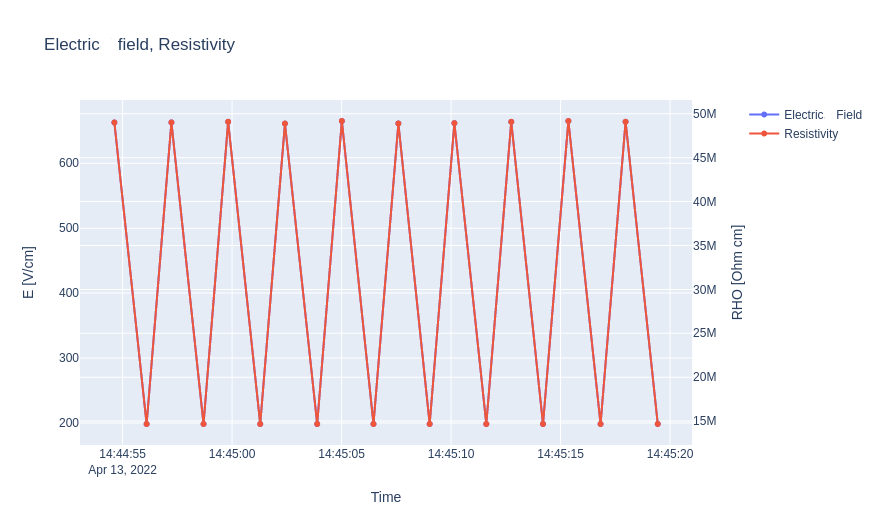
\includegraphics{CA12X_C5-3_5.png}
\caption{CA12X\_C5}
\end{figure}

Presenza ancora delle oscillazioni nell'esperimento
CA12X\_C5\_at\_fixed\_current\_4e-7A-20220413143802 con corrente
costante di \textbf{0.4uA}

\begin{figure}
\centering
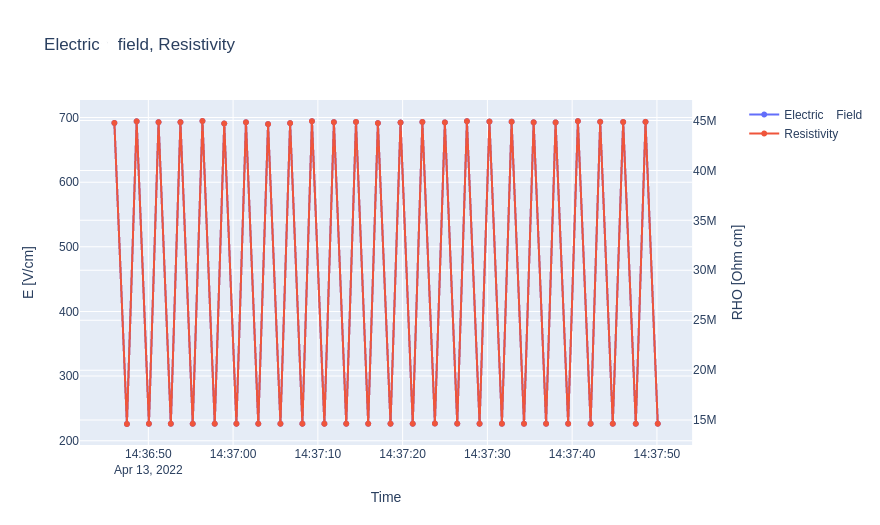
\includegraphics{CA12X_C5-4.png}
\caption{CA12X\_C5}
\end{figure}

Presenza ancora delle oscillazioni nell'esperimento
CA12X\_C5\_at\_fixed\_current\_4.5e-7A-20220413144649 con corrente
costante di \textbf{0.45uA}

\begin{figure}
\centering
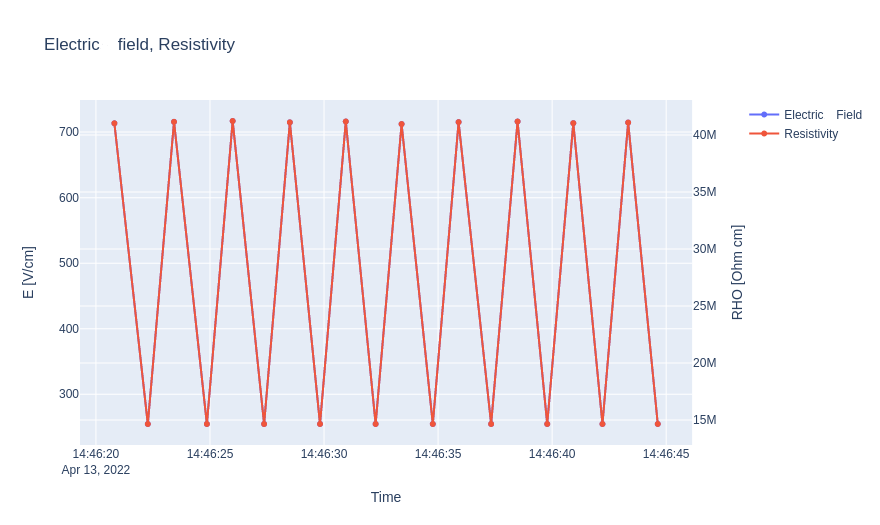
\includegraphics{CA12X_C5-4_5.png}
\caption{CA12X\_C5}
\end{figure}

Asenza di oscillazioni nell'esperimento
CA12X\_C5\_at\_fixed\_current\_5e-7A-20220413144412 con corrente
costante di \textbf{0.5uA}

\begin{figure}
\centering
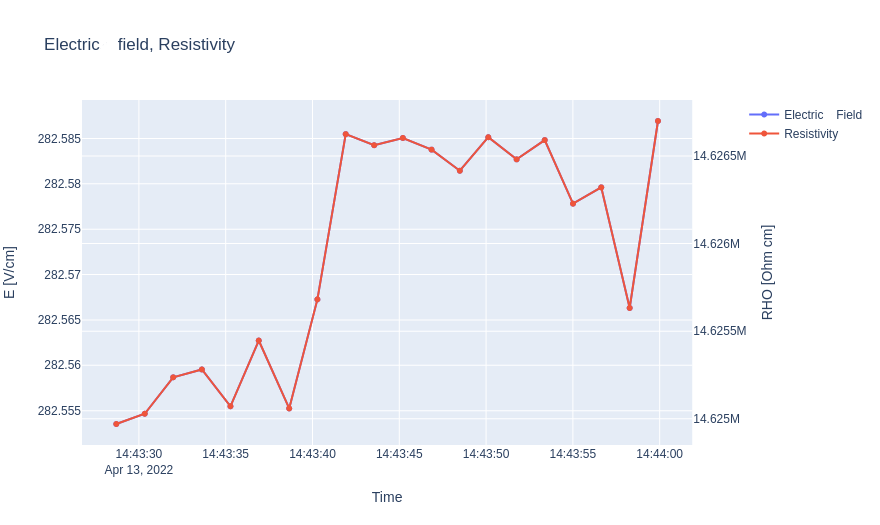
\includegraphics{CA12X_C5-5.png}
\caption{CA12X\_C5}
\end{figure}

Si riscontra la stessa modalità di comportamento polarizzando con una
rampa il campione nelle stesse condizioni di temperatura di
\textbf{113°K}

Esperimento CA12X\_C5\_current\_from\_1e-7\_to\_3.5e-7A-20220413145630
con rampa \textbf{0.1uA -\textgreater{} 0.35uA}, avvio delle
oscillazioni per corrente \textbf{\textgreater0.2uA}

\begin{figure}
\centering
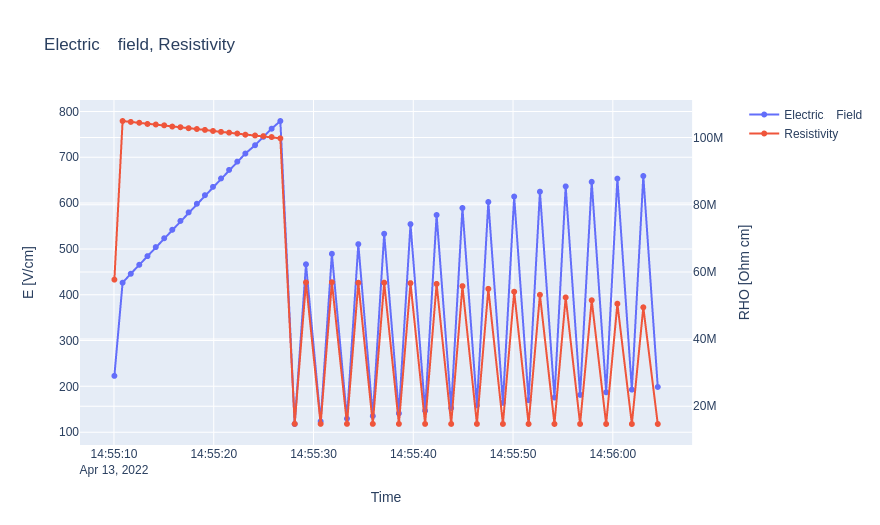
\includegraphics{CA12X_C5-1-3_5.png}
\caption{CA12X\_C5}
\end{figure}

Esperimento CA12X\_C5\_current\_from\_3.5e-7\_to\_5e-7A-20220413145837
con rampa \textbf{0.35uA -\textgreater{} 0.5uA}, arresto delle
oscillazioni per corrente \textbf{\textgreater0.45uA}

\begin{figure}
\centering
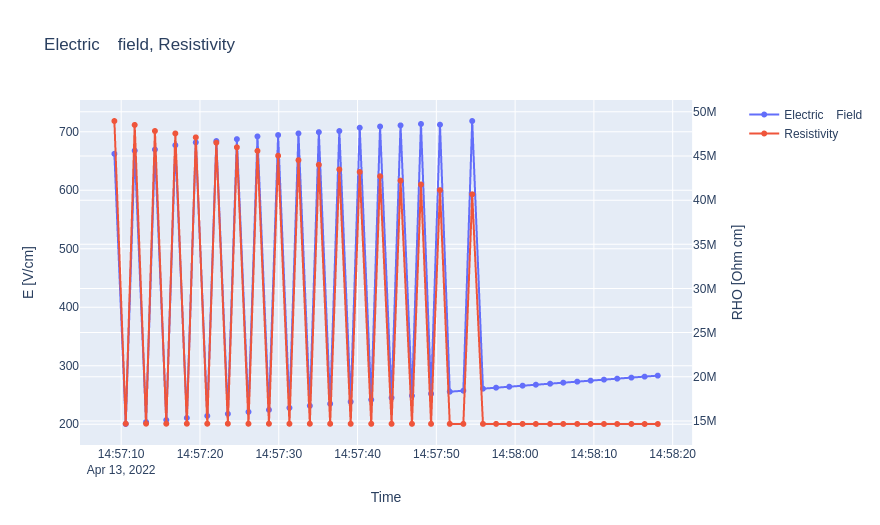
\includegraphics{CA12X_C5-3_5-5.png}
\caption{CA12X\_C5}
\end{figure}

Si possono vedere i dettagli degli esperimenti citati nella sezione 2.

    \hypertarget{finale-inatteso}{%
\subsubsection{Finale inatteso}\label{finale-inatteso}}

Osservando gli esperimenti dei paragrafi 1.3.1 e 1.3.2 relativi agli
inneschi, si nota che al termine della fase oscillatoria il campo
elettrico si assesta al valore più basso raggiunto durante questa fase,
col segnale a rampa è evidente visivamente.

Un altro esempio con rampe di corrente ripetute relativo al campione
\textbf{CA12X2\_C1} nell'esperimento
CA12X2\_C1\_current\_from\_0.5e-6\_to\_1e-6A-20220428154754

\begin{figure}
\centering
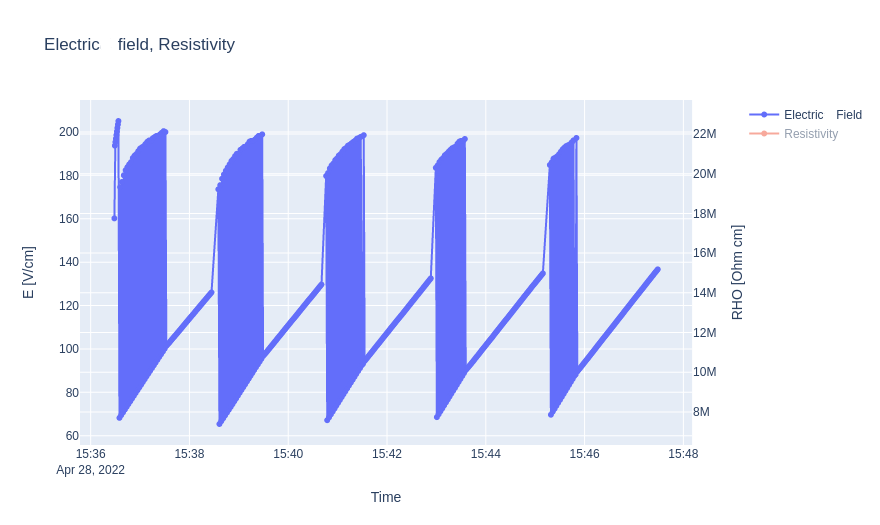
\includegraphics{CA12X2_C1-e.png}
\caption{CA12X2\_C1}
\end{figure}

\begin{figure}
\centering
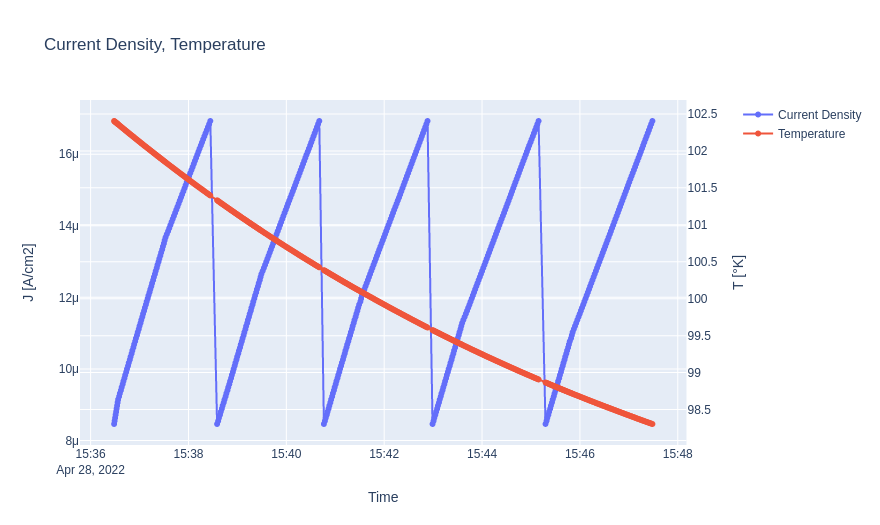
\includegraphics{CA12X2_C1-j_t.png}
\caption{CA12X2\_C1}
\end{figure}

Dettaglio delle oscillazioni della prima rampa

\begin{figure}
\centering
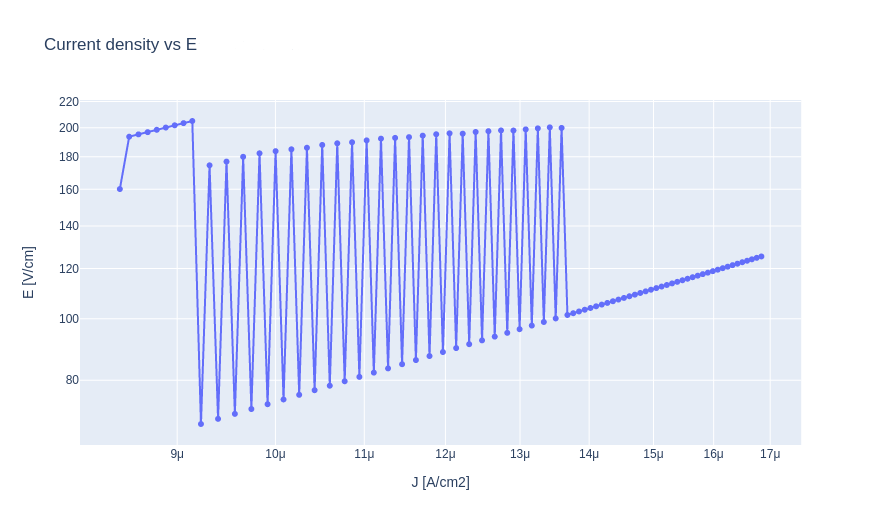
\includegraphics{CA12X2_C1-e_j.png}
\caption{CA12X2\_C1}
\end{figure}

La fase oscillatoria introduce una discontinuità di comportamento tale
da avere un campo elettrico inferiore a quello pre-oscillatorio sebbene
le correnti siano maggiori.

    \hypertarget{stati-indipendenti}{%
\subsubsection{Stati Indipendenti}\label{stati-indipendenti}}

Nella sequenza degli esperimenti a corrente costante del paragrafo 1.3.2
il comportamento è equivalente alla rampa dello stesso paragrafo. Però,
rispetto alla rampa, la sequenza degli incrementi di corrente non è
stata applicata in ordine cronologico:

\begin{longtable}[]{@{}lll@{}}
\toprule
Ordine Cronologico & Corrente {[}uA{]} & Campo {[}V/cm{]}\tabularnewline
\midrule
\endhead
2 & 0.1 & 408\tabularnewline
3 & 0.2 & 768\tabularnewline
4 & 0.3 & osc. min 170, max 620\tabularnewline
6 & 0.35 & osc. min 198, max 663\tabularnewline
1 & 0.4 & osc. min 226, max 692\tabularnewline
7 & 0.45 & osc. min 255, max 716\tabularnewline
5 & 0.5 & 283\tabularnewline
\bottomrule
\end{longtable}

Il valore finale di 0.5uA è applicato prima dei valori 0.35uA e 0.45uA.
La risposta del cristallo appare quasi deterministica e non sembra
dipendere dallo stato precedente.

    \hypertarget{simmetria-e-specularituxe0}{%
\subsubsection{Simmetria e
Specularità}\label{simmetria-e-specularituxe0}}

Esempi di esperimenti che evidenziano la caratteristica di specularità e
di simmetria del fenomeno.

L'esperimento
CA8\_01\_A\_square\_waveform\_value\_3.5e-08A-20220413144649 con
sorgente di corrente a onda quadra simmetrica di \textbf{0.035uA} mostra
questo comportamento:

\begin{figure}
\centering
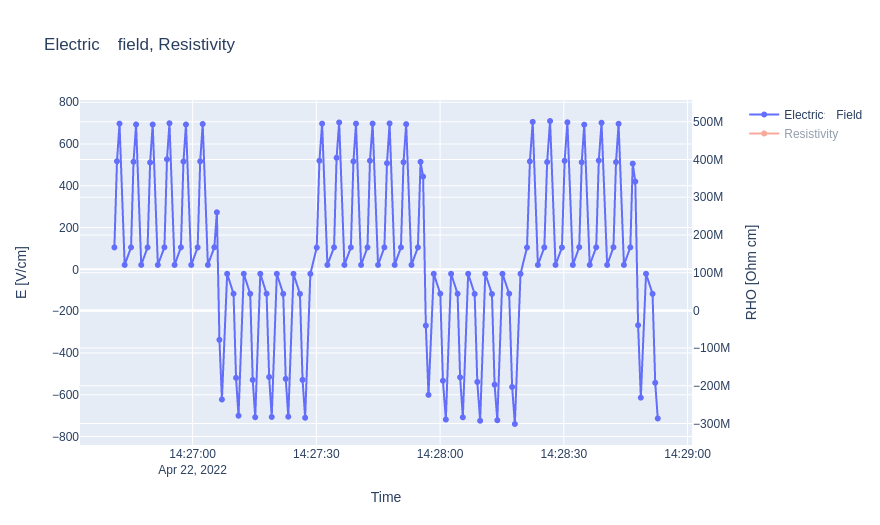
\includegraphics{CA8_01_A_square-e.png}
\caption{CA8\_01\_A\_square\_waveform}
\end{figure}

\begin{figure}
\centering
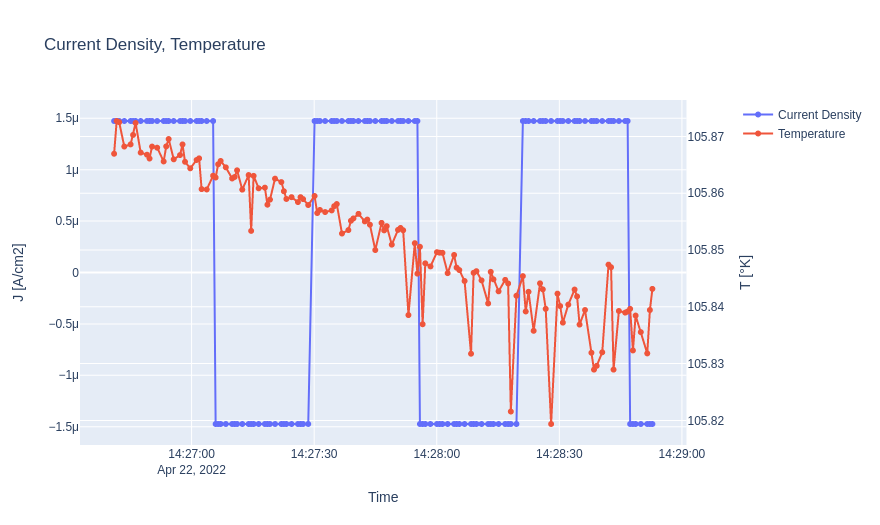
\includegraphics{CA8_01_A_square-j_t.png}
\caption{CA8\_01\_A\_square\_waveform}
\end{figure}

Gli esperimenti seguenti con forma d'onda triangolare mostrano
caratteristiche di specularità:

Esperimento
CA12X2\_current\_from\_1e-9\_to\_1000e-9A\_flipped-20220315170952

\begin{figure}
\centering
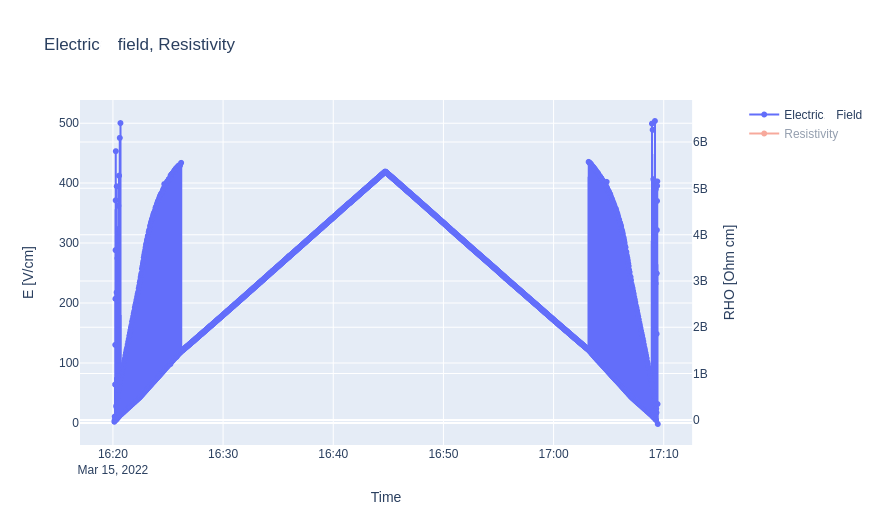
\includegraphics{CA12X2_flipped-e.png}
\caption{CA12X2\_flipped}
\end{figure}

\begin{figure}
\centering
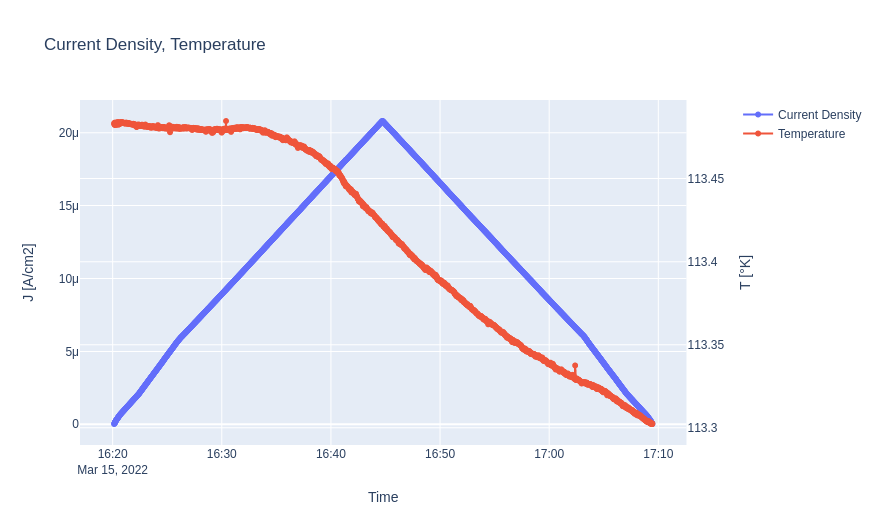
\includegraphics{CA12X2_flipped-j_t.png}
\caption{CA12X2\_flipped}
\end{figure}

Esperimento
CA12X2\_current\_from\_10e-9\_to\_100e-9A\_flipped-20220315155945

\begin{figure}
\centering
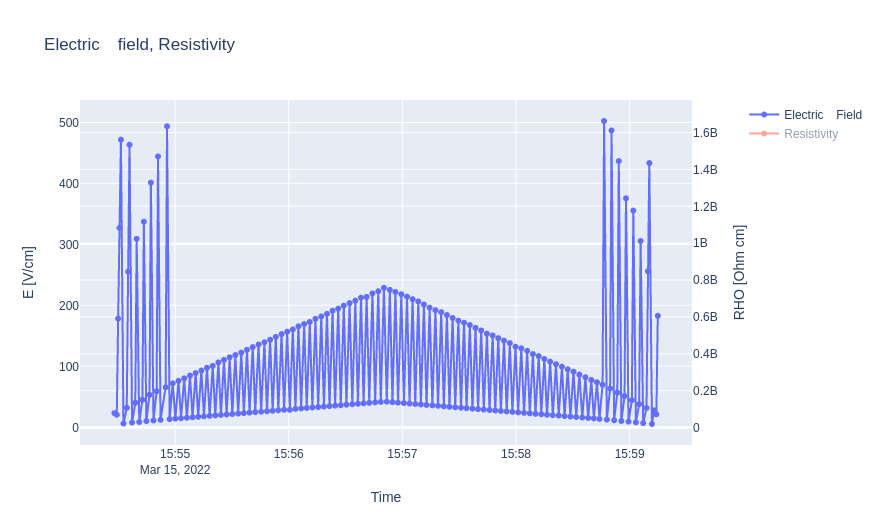
\includegraphics{CA12X2_flipped-e-1.png}
\caption{CA12X2\_flipped}
\end{figure}

\begin{figure}
\centering
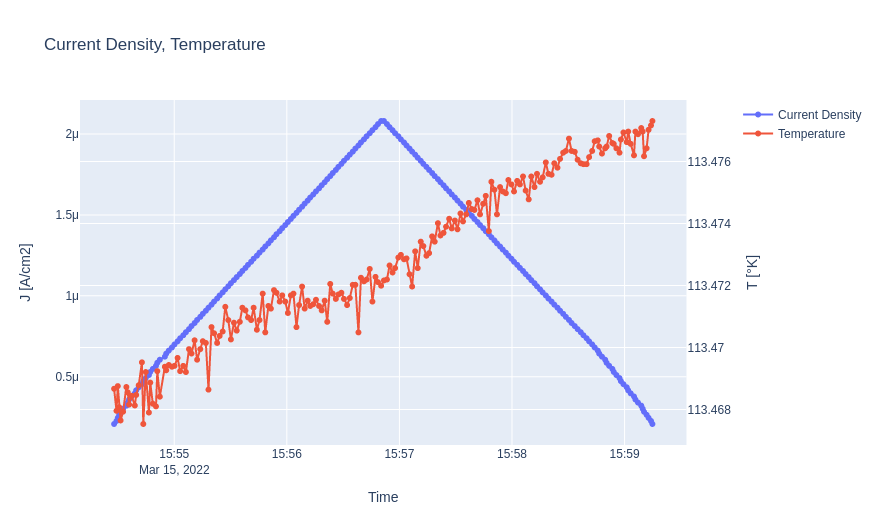
\includegraphics{CA12X2_flipped-j_t-1.png}
\caption{CA12X2\_flipped}
\end{figure}

Questi andamenti sembrano confermare le deduzioni del paragrafo 1.3.4

    \hypertarget{discontinuituxe0}{%
\subsubsection{Discontinuità}\label{discontinuituxe0}}

Quando non si innescano le oscillazioni appaiano dei salti, succede così
per il campione \textbf{CA12X2\_C3} sottoposto a una sequenza di onde
triangolari da \textbf{1uA} con picco a \textbf{12uA} a temperature
decrescenti nell'esperimento
CA12X2\_C3\_current\_from\_1e-6\_to\_12e-6A\_flipped-20220404182243:

Temperatura di \textbf{116°K}, nessun salto evidente

\begin{figure}
\centering
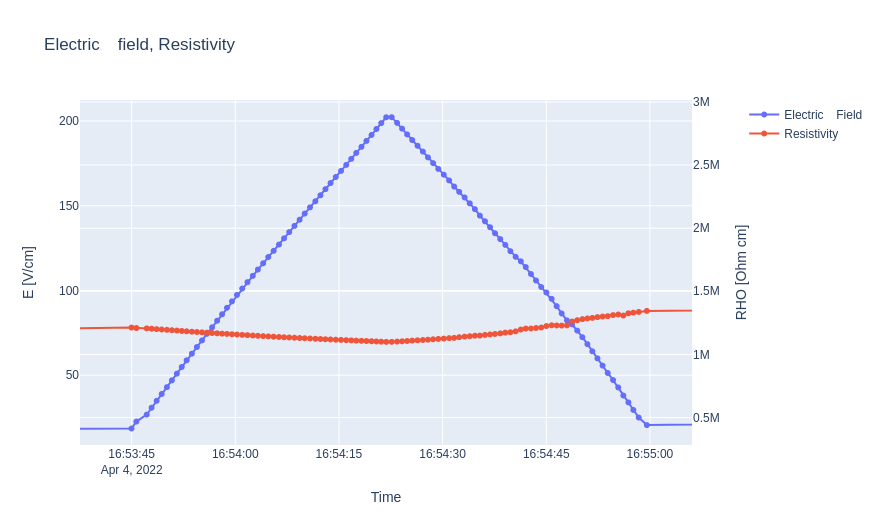
\includegraphics{CA12X2_C3-116.png}
\caption{CA12X2\_C3-1}
\end{figure}

Temperatura di \textbf{109°K}

\begin{figure}
\centering
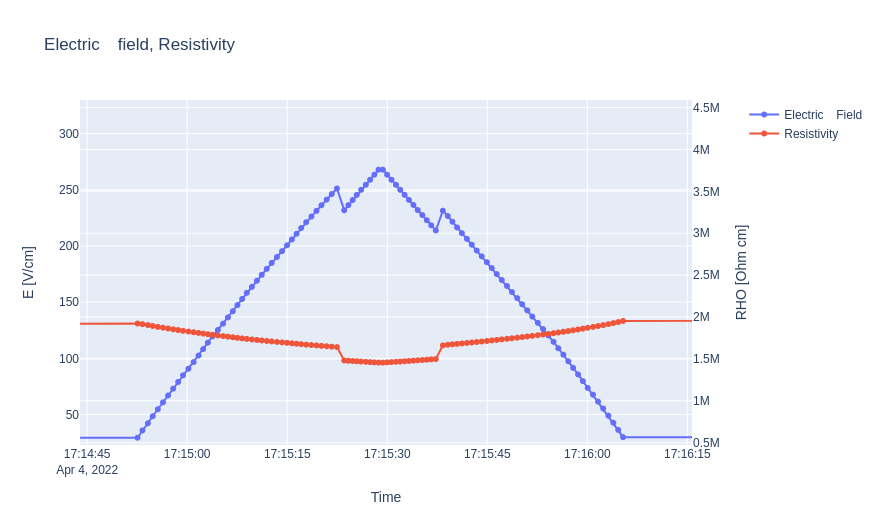
\includegraphics{CA12X2_C3-109.png}
\caption{CA12X2\_C3-2}
\end{figure}

Temperatura di \textbf{92°K}

\begin{figure}
\centering
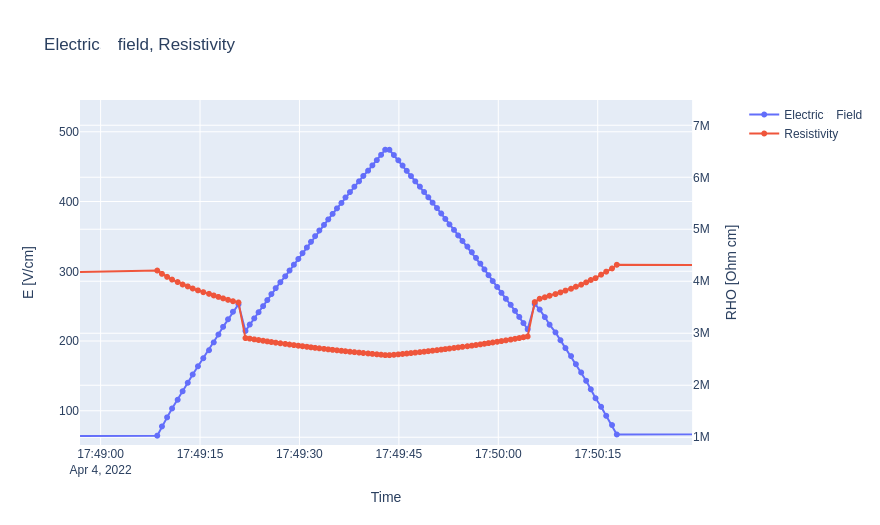
\includegraphics{CA12X2_C3-92.png}
\caption{CA12X2\_C3-3}
\end{figure}

Temperatura di \textbf{83°K}

\begin{figure}
\centering
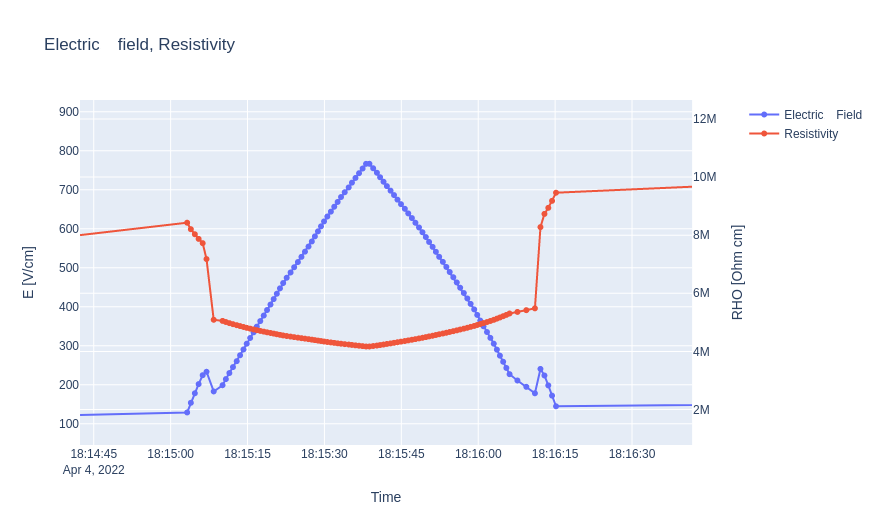
\includegraphics{CA12X2_C3-83.png}
\caption{CA12X2\_C3-4}
\end{figure}

Allo scendere della temperatura i salti avvengono a correnti più basse
come per gli inneschi delle oscillazioni

    \hypertarget{cronologia-degli-esperimenti}{%
\subsection{Cronologia degli
esperimenti}\label{cronologia-degli-esperimenti}}



    
    
    \begin{center}
    \adjustimage{max size={0.9\linewidth}{0.9\paperheight}}{output_13_1.pdf}
    \end{center}
    { \hspace*{\fill} \\}
    
    \hypertarget{distribuzione-degli-esperimenti}{%
\subsection{Distribuzione degli
esperimenti}\label{distribuzione-degli-esperimenti}}


    \begin{center}
    \adjustimage{max size={0.9\linewidth}{0.9\paperheight}}{output_16_0.pdf}
    \end{center}
    { \hspace*{\fill} \\}
    
    \hypertarget{esperimenti-con-oscillazioni}{%
\section{Esperimenti con
Oscillazioni}\label{esperimenti-con-oscillazioni}}

    Dettaglio degli esperimenti sui campioni che hanno presentato
oscillazioni del campo elettrico.


    
    
    \hypertarget{analisi-delle-oscillazioni}{%
\section{Analisi delle Oscillazioni}\label{analisi-delle-oscillazioni}}

    Analisi delle oscillazioni del campo elettrico riscontrate negli
esperimenti confrontando ampiezza e periodo in funzione di temperatura e
della sorgente di corrente.

    \hypertarget{analisi-degli-esperimenti-a-corrente-costante}{%
\subsection{Analisi degli Esperimenti a Corrente
costante}\label{analisi-degli-esperimenti-a-corrente-costante}}



    \begin{center}
    \adjustimage{max size={0.9\linewidth}{0.9\paperheight}}{output_26_0.pdf}
    \end{center}
    { \hspace*{\fill} \\}
    
    \hypertarget{oscillazioni-in-funzione-della-temperatura}{%
\subsubsection{Oscillazioni in funzione della
temperatura}\label{oscillazioni-in-funzione-della-temperatura}}

    \begin{center}
    \adjustimage{max size={0.9\linewidth}{0.9\paperheight}}{output_28_0.pdf}
    \end{center}
    { \hspace*{\fill} \\}
    
    \begin{center}
    \adjustimage{max size={0.9\linewidth}{0.9\paperheight}}{output_28_1.pdf}
    \end{center}
    { \hspace*{\fill} \\}
    
    \hypertarget{oscillazioni-in-funzione-della-corrente}{%
\subsubsection{Oscillazioni in funzione della
corrente}\label{oscillazioni-in-funzione-della-corrente}}


    \begin{center}
    \adjustimage{max size={0.9\linewidth}{0.9\paperheight}}{output_30_0.pdf}
    \end{center}
    { \hspace*{\fill} \\}
    
    \begin{center}
    \adjustimage{max size={0.9\linewidth}{0.9\paperheight}}{output_30_1.pdf}
    \end{center}
    { \hspace*{\fill} \\}
    
    \hypertarget{periodo-vs-ampiezza}{%
\subsubsection{Periodo vs Ampiezza}\label{periodo-vs-ampiezza}}


    \begin{center}
    \adjustimage{max size={0.9\linewidth}{0.9\paperheight}}{output_32_0.pdf}
    \end{center}
    { \hspace*{\fill} \\}
    
    \hypertarget{distribuzione-delle-oscillazioni-in-funzione-di-corrente-e-temperatura}{%
\subsubsection{Distribuzione delle oscillazioni in funzione di corrente
e
temperatura}\label{distribuzione-delle-oscillazioni-in-funzione-di-corrente-e-temperatura}}



    \begin{center}
    \adjustimage{max size={0.9\linewidth}{0.9\paperheight}}{output_34_0.pdf}
    \end{center}
    { \hspace*{\fill} \\}
    
    \begin{center}
    \adjustimage{max size={0.9\linewidth}{0.9\paperheight}}{output_34_1.pdf}
    \end{center}
    { \hspace*{\fill} \\}
    
    \hypertarget{analisi-degli-esperimenti-a-corrente-variabile}{%
\subsection{Analisi degli Esperimenti a Corrente
variabile}\label{analisi-degli-esperimenti-a-corrente-variabile}}


    \hypertarget{distribuzione-degli-esperimenti-in-funzione-della-temperatura-e-della-corrente}{%
\subsubsection{Distribuzione degli esperimenti in funzione della
temperatura e della
corrente}\label{distribuzione-degli-esperimenti-in-funzione-della-temperatura-e-della-corrente}}


    \begin{center}
    \adjustimage{max size={0.9\linewidth}{0.9\paperheight}}{output_38_0.pdf}
    \end{center}
    { \hspace*{\fill} \\}
    
    \hypertarget{oscillazioni-in-funzione-della-temperatura}{%
\subsubsection{Oscillazioni in funzione della
temperatura}\label{oscillazioni-in-funzione-della-temperatura}}



    \begin{center}
    \adjustimage{max size={0.9\linewidth}{0.9\paperheight}}{output_40_0.pdf}
    \end{center}
    { \hspace*{\fill} \\}
    
    \begin{center}
    \adjustimage{max size={0.9\linewidth}{0.9\paperheight}}{output_40_1.pdf}
    \end{center}
    { \hspace*{\fill} \\}
    
    \hypertarget{oscillazioni-in-funzione-della-corrente}{%
\subsubsection{Oscillazioni in funzione della
corrente}\label{oscillazioni-in-funzione-della-corrente}}

 
    \begin{center}
    \adjustimage{max size={0.9\linewidth}{0.9\paperheight}}{output_42_0.pdf}
    \end{center}
    { \hspace*{\fill} \\}
    
    \begin{center}
    \adjustimage{max size={0.9\linewidth}{0.9\paperheight}}{output_42_1.pdf}
    \end{center}
    { \hspace*{\fill} \\}
    
    \hypertarget{periodo-vs-ampiezza}{%
\subsubsection{Periodo vs Ampiezza}\label{periodo-vs-ampiezza}}

    \begin{center}
    \adjustimage{max size={0.9\linewidth}{0.9\paperheight}}{output_44_0.pdf}
    \end{center}
    { \hspace*{\fill} \\}
    
    \hypertarget{distribuzione-delle-oscillazioni-in-funzione-di-corrente-e-temperatura}{%
\subsubsection{Distribuzione delle oscillazioni in funzione di corrente
e
temperatura}\label{distribuzione-delle-oscillazioni-in-funzione-di-corrente-e-temperatura}}


    \begin{center}
    \adjustimage{max size={0.9\linewidth}{0.9\paperheight}}{output_46_0.pdf}
    \end{center}
    { \hspace*{\fill} \\}
    
    \begin{center}
    \adjustimage{max size={0.9\linewidth}{0.9\paperheight}}{output_46_1.pdf}
    \end{center}
    { \hspace*{\fill} \\}
    
    \hypertarget{correlazioni}{%
\section{Correlazioni}\label{correlazioni}}

    Calcolo della matrice di correlazione delle grandezze di ciascun
esperimento durante il fenomeno dell'oscillazione.

I valori rappresentati sono compresi tra -1 e 1. Il valore 1 indica la
massima correlazione positiva, le grandezze crescono all'unisono; il
valore -1 anch'esso è indice di una perfetta correlazione dove
l'incremento dell'una corrisponde un decremento di pari misura
dell'altra. Un valore assoluto maggiore di 0.6 è considerato un indice
di buona correlazione.

    \hypertarget{esperimenti-con-corrente-costante}{%
\subsection{Esperimenti con corrente
costante}\label{esperimenti-con-corrente-costante}}

    \begin{center}
    \adjustimage{max size={0.9\linewidth}{0.9\paperheight}}{output_51_0.pdf}
    \end{center}
    { \hspace*{\fill} \\}
    
    \hypertarget{esperimenti-con-corrente-variabile}{%
\subsection{Esperimenti con corrente
variabile}\label{esperimenti-con-corrente-variabile}}


    \begin{center}
    \adjustimage{max size={0.9\linewidth}{0.9\paperheight}}{output_54_0.pdf}
    \end{center}
    { \hspace*{\fill} \\}
    
    \hypertarget{Diffrattogrammi_a_raggi_X}{%
\section{Diffrattogrammi a raggi X}\label{Diffrattogrammi_a_raggi_X}}

    \begin{center}
    \adjustimage{max size={0.95\linewidth}{0.95\paperheight}}{analisi_rxd.pdf}
    \end{center}
    { \hspace*{\fill} \\}

    % Add a bibliography block to the postdoc
    
    
    
\end{document}
